%
% Example file
%

\documentclass{fose2019}           % for pLaTeX2e
%\documentclass[english]{fose2016} % for English papers
%\documentclass[ascii]{fose2016}   % for ASCII pTeX

\usepackage[dvipdfmx]{graphicx}
%\usepackage{epsfig}
\usepackage{comment}
\usepackage{graphicx}
\usepackage{multirow}
\usepackage{tabularx}



\title{類似コード検出ツールを用いたテストコード再利用に向けた調査}
\etitle{Investigation for Test Code Reuse Using Similar Code Detection Tool}
\journalhead{An example of use for fose2019.cls}
\author{倉地 亮介}{Ryosuke Kurachi, 奈良先端科学技術大学院大学}
\author{崔 恩瀞}{Eunjong Choi, 京都工芸繊維大学}
\author{飯田 元}{Hajimu Iida, 奈良先端科学技術大学院大学}

\begin{document}

\maketitle


\begin{abstract}
本研究では,既存のテストコードの再利用によるテストコード生成環境の実現に向けて,類似するプロダクトコードのペアを分類し,類似コードペア間とテストコードペア間の類似度の関係を調査した.
\end{abstract}

\section{はじめに}
テスト工程において,テスト作成コストを削減するために様々なテストコード自動生成ツールが提案されてきた.しかし,既存のツールによって生成されるテストコードはテスト対象コードの作成経緯や意図に基づいていないという性質から開発者の保守作業を困難にするという課題がある\cite{ICST}.この課題の解決方法として既存テストの再利用によるテストコード生成を行う環境が有効であると考えられる.

\indent 提案環境では,類似コード検出ツールを用いてテスト生成対象のコード片aに対して類似したコード片を検出する.そして,類似コード片に対応するテストコードを再利用することでコード片aのテストコードを生成する.

\indent 既存テストの再利用は,命名規則に従った保守性の高いテストコードの生成が期待できる.一方で,類似コード間でのテスト再利用は,適用対象の類似コードペアが存在する必要があることや,テスト対象となる類似コードペア間の関係に依存するので困難な作業である.そのため,どのようなテストコードが類似コード間で再利用できるのかを明らかにすることがテストコードの再利用支援において重要である.

\indent 本研究は提案環境の開発に向けてプロジェクト内の類似コードペアをテストコードの有無によって分類し,「両方のコード片にテストコードが存在する類似コードペア」を対象に類似コードペア間とテストコードペア間の類似度の関係を調査した.

\begin{comment}
その結果,類似コードペアの類似度とテストコードの類似度には相関があることが分かった.
\end{comment}

\section{調査概要}
\subsection{調査方法}
類似コードペアをテストコードの有無によって分類し,類似コードペア間とテストコードペア間の類似度の関係を調査する.調査手法はまず,OSS上の有名な3つのJavaプロジェクト内のテストコードとプロダクトコードをそれぞれ抽出し,類似コード検出ツールNICADを用いて類似コードペアを検出した\cite{ICPC}.次に,類似コードペアのテストコードを特定し,テストコードの有無によって類似コードペアを分類した.そして「両方のコード片にテストコードが存在する類似コードペア」を対象にソースコードの類似度を差異の度合いを表すタイプ\cite{SCP}によって計算した.
\begin{comment}
\begin{figure}[htbp]
  \centering
  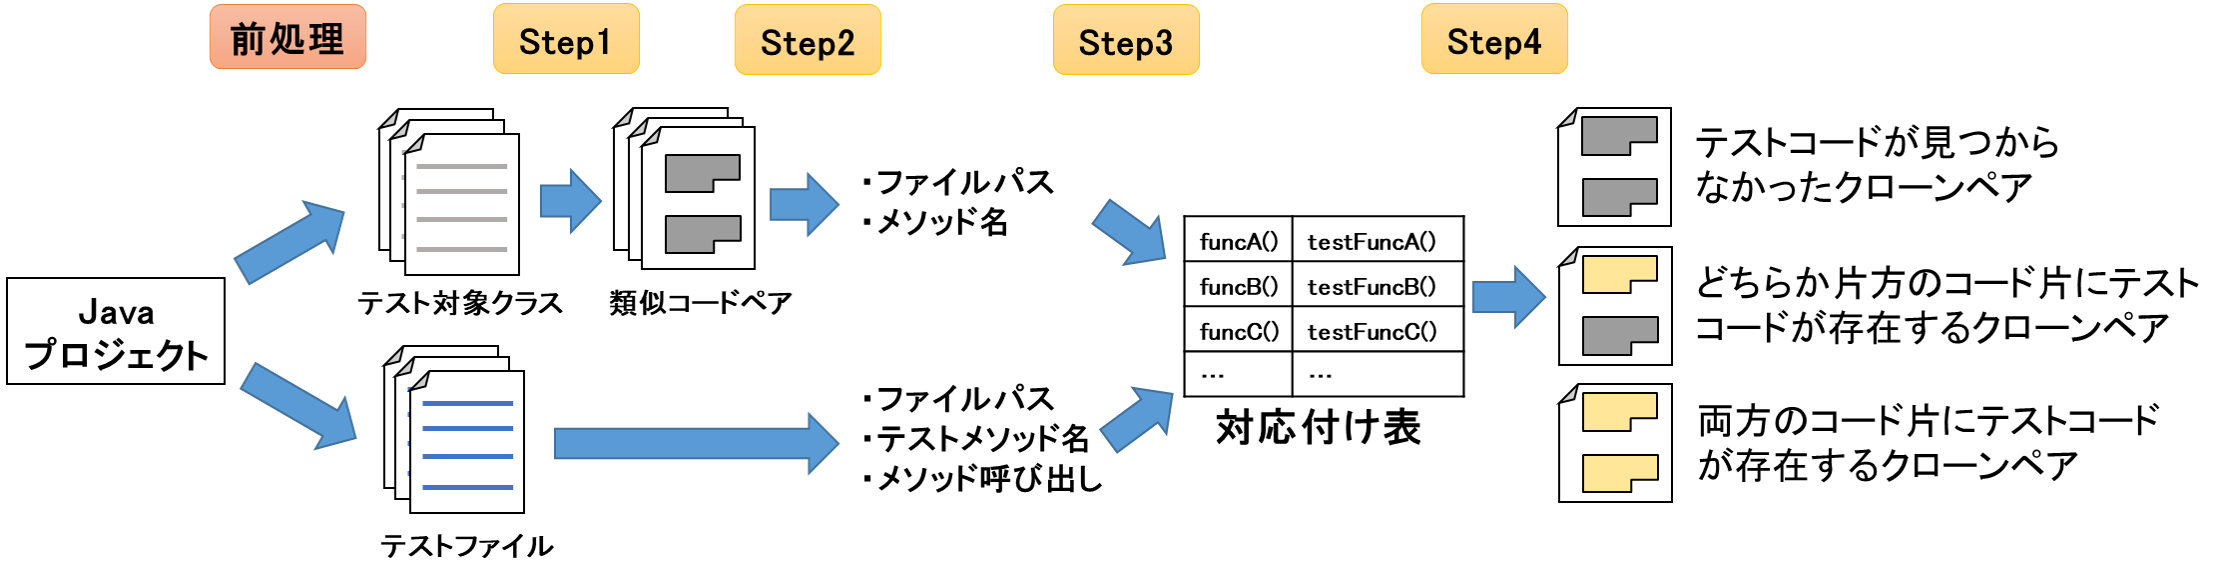
\includegraphics[width=\textwidth]{2.png}
%  
\epsfig{file=fose2005logo.eps,width=\textwidth}
  \caption{類似コードペアの分類手法の概要}
  \label{fig:example}
\end{figure}
\end{comment}
%\section{調査概要}
%\begin{comment}
%\begin{description}
%\item[調査1:]プロジェクト内にテストの再利用候補となる類似コードのペアはどの程度存在するか
%OSSに存在する人気javaプロジェクトを対象に調査を実施し,類似コード間のテスト再利用手法がどの程度有効なのかを明らかにする
%\item[調査2:]類似コードペア間の類似度と対応するテストコードペア間の類似度にはどのような関係があるか
%テストコード間の類似度が高いほど再利用できる可能性も高くなると考えられるので,
%「両方のコード片にテストコードが存在する類似コードペア」を対象に類似コードペアの類似度とテストコードの類似度をソースコードの差異の度合いを示すタイプ別に分類し関係性を調査
%\end{description}
%\end{comment}

\begin{table}[]
\centering
\caption{既存Javaプロジェクト中の類似コードペアの分類結果}
\label{table1}
\begin{tabular}{|p{3.5em}|c|p{4em}|c|p{2.5em}|c|c|l|}
\hline
\multicolumn{2}{|c|}{}                     & \multicolumn{2}{c|}{}                     & \multicolumn{2}{c|}{}                     & \multicolumn{2}{c|}{}                         \\
\multicolumn{2}{|c|}{\multirow{-2}{*}{\begin{tabular}[c]{@{}c@{}}\scriptsize 両方のコード片にテストコード\\ \scriptsize が存在する類似コードペア\end{tabular}}} & \multicolumn{2}{c|}{\multirow{-2}{*}{\begin{tabular}[c]{@{}c@{}}\scriptsize どちらか片方のコード片にテスト\\ \scriptsize コードが存在する類似コードペア\end{tabular}}} & \multicolumn{2}{c|}{\multirow{-2}{*}{\begin{tabular}[c]{@{}c@{}}\scriptsize テストコードが存在\\ \scriptsize しない類似コードペア\end{tabular}}} & \multicolumn{2}{c|}{\multirow{-2}{*}{\scriptsize 合計}}     \\ \hline
\scriptsize \hfil 数 \hfil                  & \scriptsize 割合(\%)                & {\scriptsize \hfil 数 \hfil}                  &\scriptsize 割合(\%)               & {\scriptsize \hfil 数 \hfil}                  & \scriptsize 割合(\%)               & \multicolumn{2}{c|}{\scriptsize 数} \\ \hline
\scriptsize \hfil 62 \hfil                 & {\scriptsize 4.9}                    &  {\scriptsize \hfil 334 \hfil}                & {\scriptsize 26.2}                 & {\scriptsize \hfil 879 \hfil}                 & {\scriptsize 68.9}                 & \multicolumn{2}{c|}{\scriptsize 1275}                     \\ \hline
\end{tabular}
\end{table}



\begin{table}[]
\centering
\caption{類似コードペア間の類似度とテストコードペア間の類似度の関係}
\label{table2}
\begin{tabular}{|c|c|c|c|c|}
\hline
                             & \multicolumn{4}{c|}{\scriptsize テストコードペア間の類似度}         \\ \hline
\multirow{4}{*}{\scriptsize 類似コードペア間の類似度} &             & \scriptsize タイプ2 & \scriptsize タイプ3 & \scriptsize Not Similar \\ \cline{2-5} 
                             & \scriptsize タイプ2 & \scriptsize 77          & \scriptsize 10     & \scriptsize 6     \\ \cline{2-5} 
                             &\scriptsize タイプ3       & \scriptsize 28           & \scriptsize 5    & \scriptsize 10    \\ \cline{2-5} 
                             & \scriptsize Not Similar       & \scriptsize 0           & \scriptsize 0    & \scriptsize 17     \\ \hline
\end{tabular}
\end{table}


\subsection{調査結果}
3つのJavaプロジェクトを対象にテストコードの有無によって類似コードペアの分類を行った結果を表\ref{table1}に示す.この表からプロジェクト中のテスト対象となる類似コードペアの内,26.2\%が既存テストを再利用できる可能性があることが分かる.すなわち,類似コードペア内で片方のコード片にはテストコードがあるにもかかわらず,もう片方のコード片はテストされていない類似コードペアが全体の4分の1以上を占めており,提案環境の実現によって多くのコード片にテストコードを再利用できる可能性を示している.
\indent 類似度の関係調査では,類似コードペアの分類によって得られた「両方のコード片にテストコードが存在する類似コードペア」62個とそれに対応するテストコードのペア153個の類似度の関係を表\ref{table2}に示した.調査の結果,テスト対象となる類似コードペアが類似していない(Not Similar)場合は,類似するテストコードペアが存在しないことが分かる.また,類似コードペアの類似度がタイプ2,3の場合は,テストコードの類似度もタイプ2,3が多い結果となった.この結果は,テストコードペアの間の類似度と対象の類似コードペア間の類似度には相関関係があり,類似コードペア間の類似度が高いほどテストコードを再利用できる可能性が高いことを示している.
\indent 一方で,類似コードペア間の類似度がタイプ2と高いにもかかわらず,テストコードペアが類似しない組み合わせが6件検出された.これらの類似コードペアのメソッドを確認したところ,同じ制御構造を持つが,最後に出力する数値の選択だけが異なっていることが分かった.検出された例として,Apache kafkaでは,同一の制御構造で特定のオブジェクトを取得した後,getメソッドでデータを取得する処理と,deleteメソッドでデータを削除する処理が類似コードペアとなっていた.このように共通のデータを使用し,互いに関係した処理であっても,異なる処理を実行している場合は,テストコードを再利用することは難しいと考えられる.そのため,類似コードペア間の振る舞いに着目して分類を行い更なる調査をする必要がある.

\section{まとめ}
本研究では,プロジェクト内の類似コードペアを分類し,類似コードペア間とテストコードペア間の類似度の関係を調査した.その結果,類似度の関係には相関があることを明らかにした.また,調査結果から類似コードペア間のタイプによる類似度だけでなく,振る舞いにも着目する必要があることが分かった.今後は,既存のメソッド呼び出しの差異に基づく類似コードペアの分類手法を用いて,類似コードペア間の振る舞いと対応するテストコードの関係を調査をする予定である.
%\bibliography{own,related,misc}

\acknowledgements{}
本研究はJSPS科研費 JP18H04094, 19K20240の助成を受けた.

\bibliographystyle{junsrt}
\begin{thebibliography}{2}
\bibitem{ICST} S. Shamshiri, et al. How Do Automatically Generated Unit Tests Influence Software Maintenance?. {\it Proc. of ICST}, pp.239--249, 2018. 
\bibitem{ICPC} C. K. Roy, et al. NICAD: Accurate Detection of Near-Miss Intentional Clones Using Flexible Pretty-Printing and Code Normalization. {\it Proc. of ICPC}, pp.172--181, 2008.
\bibitem{SCP} C. K. Roy, et al. Comparison and evaluation of code clone detection techniques and tools: a qualitative approach. Science of Computer Programming, Vol. 74, No. 7, pp. 470–495, 2009.
%\bibitem{fose2019} 伊藤 恵,神谷 年洋 編:ソフトウェア工学の基礎XXVI,
%     日本ソフトウェア科学会{\em FOSE2019}, 近代科学社, 2019. (to appear)
\end{thebibliography}



\end{document}
